\section{Introduction}
\label{section:intro}
In this report, we will provide the results of a careful investigation of the performance of a variety of software packages applied to typical initial value ordinary differential equation (IVODEs) encountered in Covid-19 models. 

For any mathematical model, the accuracy requirements of the numerical solution should be determined by the quality of the model and the accuracy of the parameters that appear in the model. Numerical errors associated with the computational techniques that are used to obtain the solution must always be negligible compared to the accuracy to which the model is defined. \emph{Researchers deserve to obtain numerically accurate solutions to the models that they are studying}. In this report, \emph{we will show that the straightforward use of standard IVODE solvers on typical Covid-19 models can lead to numerical solutions that have large errors, some of the same order of magnitude as the solution itself.} Most of the IVODE solvers that we consider in this report allow the user to specify a parameter called a tolerance. The solvers use adaptive algorithms to attempt to compute an approximate solution with a corresponding error estimate that is approximately equal to the tolerance.

In Section $\ref{subsection:research_papers}$, we review examples of how IVODEs are used in epidemiology. In Section $\ref{subsection:SEIR_model}$, we define the SEIR models which we will consider throughout this report; in Section $\ref{subsection:exponential_growth}$, we discuss the problem of stability as it concerns problems with exponentially growing solutions; in Section $\ref{subsection:fixed_vs_control}$, we explain the difference between fixed step-size and error-controlled IVODE solvers. The IVODE software packages from programming environments that are typically used by researchers are described in Section $\ref{subsection:numerical_software_used}$. We also make a note of issues with evaluation at output points that lead to inefficiencies for some of these solvers in Section $\ref{subsection:solution_output_points_impl}$. In Section $\ref{subsection:effect_of_discontinuity}$, we discuss the effects of problem discontinuities on the performance of these solvers.

In Section $\ref{subsection:naive_time_problem}$, we apply the solvers to a Covid-19 problem with a time-dependent discontinuity and show how this results in numerical solutions with relative errors of the same magnitude as the solution we are trying to compute. In Section $\ref{subsection:time_disc_handling}$, we will use discontinuity handling to accurately solve the time-dependent problem. In Section $\ref{subsection:time_tolerance_study}$, we will use a range of tolerances to discuss the effects of tolerance on the accuracy and efficiency of some of the solvers.

In Section $\ref{subsection:naive_state_problem}$, we apply the solvers to a Covid-19 problem with a state-dependent discontinuity and show how none of the solvers can obtain accurate solutions. We will explain how even the use of very sharp tolerances is not sufficient to improve the computed solutions in Section $\ref{subsection:state_sharp_tol_failed}$ and show that the only effective way to solve this problem is through event detection, which we will describe in Section $\ref{subsection:intro_event_detection}$. We then show an accurate solution to the problem in Section $\ref{subsection:state_with_event_detection}$ and perform a tolerance study on this problem in Section $\ref{subsection:state_tolerance_study}$.

In Section $\ref{section:fortran_inaccuracies}$, we examine implementation details for solvers with exceptionally poor solutions to investigate the cause of their errors. We conclude the report in Section $\ref{section:summary}$ with a summary and a discussion of the potential for future work projects.

\subsection{Epidemiological modelling}
\label{subsection:research_papers}
One common form of an epidemiological study is forecasting. Using previously obtained parameters, the researcher develops a mathematical model involving differential equations which are solved using an ODE solver. Often, the solver will be used to integrate over a large time period so that the researcher can examine how the disease will spread. For such problems, sharp tolerance values should be used and the solver-problem combination is expected to be resilient over large time periods. In Section $\ref{subsection:exponential_growth}$, we discuss why it is unrealistic to attempt to compute a numerical solution for large time periods if the infection is still growing exponentially and how measures such as social distancing allow solvers to reduce errors so that reasonably accurate solutions can be computed over longer time periods.

A second type of epidemiology study involves parameter estimation. In this kind of study, data points are collected about the spread of a virus and we try to fit a mathematical model to that data. In so doing, we can estimate the parameters’ values that will minimize the error in the fit. An example of such a study can be found in Appendix $\ref{section:ebola_paper}$. Parameter estimation studies often involve using an ODE solver inside an optimization algorithm and thus the computing time, especially for large problems, can be significant. The computational cost being typically inversely proportional to the tolerance, we will investigate to what extent coarse tolerances can be employed in the computation of solutions to Covid-19 models.

\subsection{Detailed description of two specific models to be considered in this report.} 
\label{subsection:SEIR_model}
In this section, we explain how an IVODE problem is defined. We then describe the models that we are going to consider in this report. They involve typical SEIR models to which we add discontinuities.
VI ==========================
(Reference Christina Christara. I DONT HAVE ONE!!!!) 
============================= VI

An IVODE problem is defined by the equations and the initial conditions:
\begin{equation}
y'(t) = f(t, y(t)), \quad y(t_0) = y_0 \nonumber
\end{equation}
where $f(t, y(t))$ is a function that defines the derivative at time, t. A complete definition also includes the initial value of the solution components. Thus given $f(t, y(t))$ and $y(t_0)$, we find approximations to  $y(t)$ using numerical methods. 

In this report, we define a Covid-19 model as follows:
\begin{equation}
\frac{\textit{d}S}{\textit{dt}} = \mu N - \mu S - \frac{\beta}{N}IS, \nonumber
\end{equation}

\begin{equation}
\frac{\textit{d}E}{\textit{dt}} = \frac{\beta}{N}IS - \alpha E - \mu E, \nonumber
\end{equation}

\begin{equation}
\frac{\textit{d}I}{\textit{dt}} = \alpha E - \gamma I - \mu I, \nonumber
\end{equation}

\begin{equation}
\frac{\textit{d}R}{\textit{dt}} = \gamma I - \mu R, \nonumber
\end{equation} 

In this SEIR model, we describe the epidemic over time. S is the number of susceptible individuals, E is the number of exposed individuals, I is the number of infected individuals and R is the number of recovered individuals at a point in time. We also use N to represent the population size.
The other parameters in this model are as follows: $\alpha$ is such that $\alpha^{-1}$ is the average incubation period, $\beta$ is the transmission rate, $\gamma$ is the recovery rate and $\mu$ is the birth/death rate. In this report, we assume that all these parameters are known as our goal is to investigate the performance of IVODE solvers on discontinuous forms of this problem. We will see that we get solutions that are not efficiently computed or that may have significant errors. This latter issue can have serious consequences as the computed solution will fail to show the actual impact of the virus as it corresponds to the actual epidemiology theories behind the mathematical models. These incorrect numerical solutions may lead epidemiologists into reaching incorrect conclusions and thus lead them into questioning the mathematical models themselves when, in fact, it is the solvers that are at fault.

The discontinuities we are going to consider involve the parameter $\beta$.
Before measures such as social distancing, masking, vaccinations, etc. are implemented, $\beta$ has a much higher value than after the measures are introduced. In our case, $\beta$ will be 0.9 before the measures and 0.005 after they are implemented corresponding to a highly contagious variant and extreme shut down measures respectively. Such an abrupt change in a modeling parameter introduces a discontinuity as we will show in Section $\ref{subsection:effect_of_discontinuity}$. We will consider two types of discontinuities. One depends only on $t$; the other depends on the value of one of the solution components. We will refer to the former as a time-dependent discontinuity and the latter as a state-dependent discontinuity.

For the time-dependent discontinuity, we will assume that at some point in time, measures are implemented that will lead to a reduction in the parameter $\beta$. We would like to solve the problem through this discontinuity but as we will show, this discontinuity introduces a numerical issue.

For the state-dependent discontinuity, we consider the following situation. If the population of exposed people reaches a certain maximum threshold, measures are introduced, which decreases the value of $\beta$. This introduces a discontinuity. Then, when the population of exposed people drops below a certain minimum threshold, the measures are relaxed, which increases $\beta$ back to its original value, which introduces another discontinuity. We will try to model this problem through multiple instances of shut-downs followed by periods where measures are relaxed. We consider a case where vaccines are not being used. This leads to setting $\beta$ back to its original value when the measures are removed. We note that each time we change the parameter $\beta$, a discontinuity is introduced and thus this problem is far more discontinuous than the previous one, which had only one discontinuity. For this problem, we show that all the solvers will fail.

The other parameters are assumed to always be constant with N = 37,741,000 (the approximate Canadian population size), $\alpha$ = 1/8, $\gamma$ = 0.06, and $\mu$ = 0.01/365. The initial values are E(0) = 103, I(0) = 1, R(0) = 0 and S(0) = N - E(0) - I(0) - R(0). This gives us a complete system of IVODEs that is in a form that can be solved by typical software packages.

\subsection{Exponential growth and the issue of instability}
\label{subsection:exponential_growth}
Some of the solution components of the SEIR model exhibit exponential growth over certain time periods. In this section, we discuss exponentially growing solutions and their impact on the computation of a numerical solution. First of all, we give a quick overview of stability for ODEs. Then we will show that the SEIR model is unstable over certain time intervals and how measures such as social distancing can improve the stability. This is important as this essentially means that before measures are implemented, accurate models are for the most part very difficult to obtain but the addition of the measures such as social distancing can give us hope that the solvers can perform better.

The stability of an ODE is associated with the impact of small changes to the initial values of the solution to the problem. An ODE is unstable if a small change in the initial values results in a significantly different solution; otherwise, the ODE is said to be stable.

It is straightforward to see that problems with a solution component that exhibits exponential growth are unstable. As mentioned above, this is the case with some of the solution components of a Covid-19 model. The population of infected people, $I$, grows exponentially as long as no measures are introduced to reduce the spread of the virus. This means that ODE solvers will experience difficulties in obtaining accurate numerical solutions. 

In Figure $\ref{fig:unstability_of_exponential_growth}$, we show exponentially growing solutions corresponding to models with slightly different initial values for E(0). We can see that we get different solutions, that become even more different as time increases.

\begin{figure}[H]
\centering
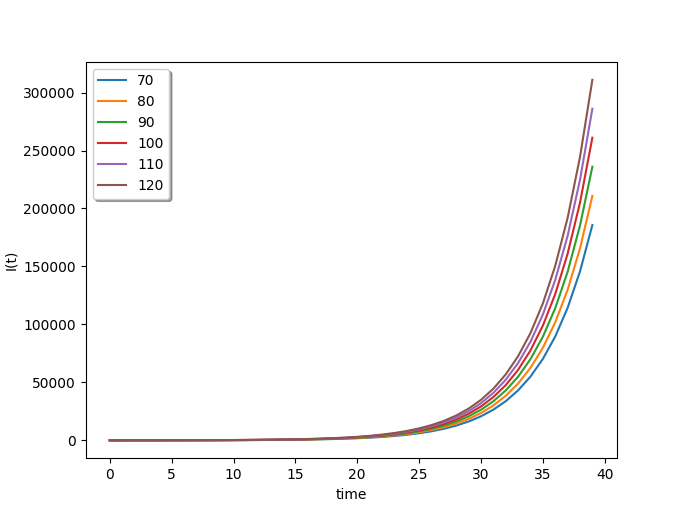
\includegraphics[width=0.7\linewidth]{./figures/unstability_of_exponential_growth}
\caption{When a solution exhibits exponential growth, relatively small changes in the initial value can eventually lead to much different solution values. Here the initial E value is 70, 80, .., 120}
\label{fig:unstability_of_exponential_growth}
\end{figure}

However, when we introduce measures such as social distancing, which leads to a smaller $\beta$ value, the problem will exhibit slower exponential growth or can even show exponential decay. A slower exponential growth means that the solution will not be as sensitive to changes to the initial values. Exponential decay is even better as the solutions from different initial values will converge.

Epidemic modeling problems exhibit solutions with this type of behavior. At first, the problem is unstable but as measures are implemented, which lead to exponential decay rather than growth, the problem becomes stable. We show this in Figure $\ref{fig:regain_stability_after_measures}$ for the problem with the time-dependent discontinuity. At first, the solutions diverge when there is exponential growth, but the introduction of measures such as social distancing introduce exponential decay which makes them converge. Thus the measures not only save lives but also improve the accuracy of the computed solutions.

\begin{figure}[H]
\centering
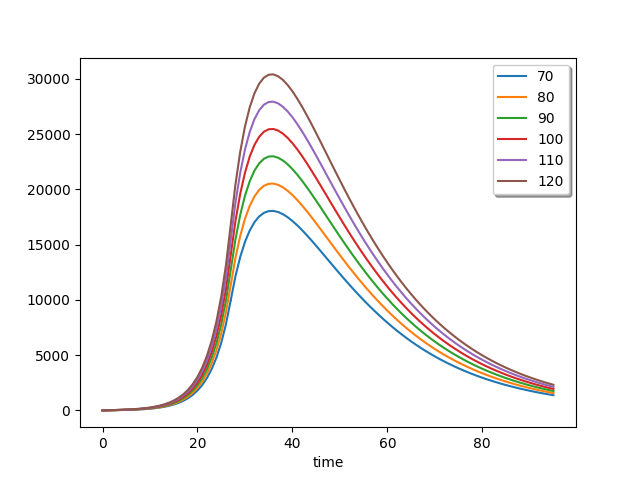
\includegraphics[width=0.7\linewidth]{./figures/regain_stability_after_measures}
\caption{Unstable solutions in the region [0, 40] becomes stable as measures are implemented in the region [40. 90]}
\label{fig:regain_stability_after_measures}
\end{figure}

\subsection{Brief overview of numerical software}
We start by explaining how solvers attempt to solve an IVODE problem. Given initial values (at the initial time, $t_0$), the solver will use an initial step size, $h$, to compute a solution at time, $t_1 (= t_0 + h)$. Similarly, the solver will attempt to take a sequence of steps until it reaches the end time. High-quality solvers will then run an interpolation algorithm usually locally within each step to get a continuous numerical solution. We note that a solver is said to have order $p$ if the difference between the true solution and the computed solution is $O(h^p)$.

In the next section, we describe what a solver will attempt to do to improve the accuracy of the computed solution. We then discuss the numerical solvers we are going to use throughout our investigation. We will then provide an additional discussion on the implementation of interpolation to get a continuous numerical solution and how certain programming environments have not updated their ODE solvers to use interpolation.

\subsubsection{Fixed Step Size and Error Control Solvers}
\label{subsection:fixed_vs_control}
In this section, we explain the role of the tolerance and the difference between fixed step size and adaptive step-size error control solvers.

The tolerance is a measure of how accurate we want the solution computed by the solvers to be. Generally, an absolute tolerance of $10^{i}$ means that we want the error estimate to be within $10^{i}$ (The computed solution has an error estimate approximately equal to the tolerance) whereas a relative tolerance of $10^{i}$ means that we want the ratio of the error estimate and the computed solution to be within $10^{i}$ (The computed solution has an error estimate where the ratio of the estimate to the computed solution is approximately equal to the tolerance). This is not always the case as some solvers will use a blended combination of the provided absolute and relative tolerances.

A solver is said to have a fixed step size if the solver begins with an initial step-size and this step-size is used throughout the whole integration. It will go from one point to another point in a `step' and will not check if the numerical solution it obtains at the end of each step is sufficiently accurate. Thus, the distance between the points, i.e, the step size, is constant throughout the computation.

An error-controlled solver starts with an initial step size but as it takes a step, it will compute an error estimate and, based on the tolerances will repeat the computation with a smaller step-size if the error estimate is larger than the tolerance. It will repeat this process until the error estimate satisfies the given tolerance. Only then will it move to the next step. Thus it reduces the step-size as needed throughout the computation. We note that the error depends on the step-size and that a smaller step-size generally leads to a smaller error. However, a small step-size means that the computation is slower because more steps will be needed and thus if the error estimate is much smaller than the tolerance, a solver will increase the step-size for the next step. This allows it to make sure that the given tolerance is satisfied over the whole problem interval and that as large a step as possible is being taken to optimize the efficiency of the computation.

Error control is not simple to implement. This is where we need to caution against the use of non-standard ODE solvers or fixed step-size solvers. Also, some researchers may be tempted to write their own solvers. These researchers often program a non-error control method like a simple fixed step-size Euler or Runge-Kutta method. We will show, using provided fixed step-size solvers in R, how these solvers simply cannot solve a Covid-19 model with reasonable accuracy. Without error control, these solvers cannot handle the discontinuity and stability issues that are present in these models and they will give very erroneous solutions, often without even a warning that the computed solutions should not be trusted.

\subsubsection{The ODE Solvers}
\label{subsection:numerical_software_used}
The ODE solvers are grouped in the following classes: Runge-Kutta methods, Runge-Kutta pairs, and multi-step methods.

A Runge-Kutta method is a one-step method that uses function evaluations, i.e, evaluations of $f(t, y(t))$, within the step. A solver based on this type of method integrates with a fixed sequence of steps and has no error control. An example is the classical four-stage, fourth-order Runge-Kutta method.

A Runge-Kutta pair uses two Runge-Kutta methods. One of the methods is used to compute a solution and the second method is used to compute an error estimate. A solver that is based on a Runge-Kutta pair resizes the step based on the error estimate, as discussed previously. An example is the DOPRI5 solver that uses a fifth-order method for the solution and a fourth-order method for the error estimate.

A multi-step method is a solver that will use a linear combination of the solutions and function values from both the current and previous steps to take the next step. An example is LSODA. Such solvers perform error estimation using two different multi-step methods. 

\subparagraph{R packages}
Scientists who solve ODE models in R commonly use the deSolve package, \cite{soetaert2010solving}, and the $ode()$ function within it.
$ode()$ provides many numerical methods to solve a problem but we have focused our investigation only on the following popular choices: `lsoda', `daspk', `euler', `rk4', `ode45', `Radau', `bdf' and `adams'. The default method is `lsoda' and the default tolerances are $10^{-6}$ for both the absolute and relative tolerances. We also note that we did not consider the other integrators in the deSolve package like $rkMethod()$, which provides other Runge-Kutta methods, and the other methods which are called by the $ode()$ function itself.

The error control solvers are:
\begin{itemize}
\item `lsoda' calls the Fortran LSODA routine from ODEPACK. It can automatically detect stiffness and choose between a stiff (BDF) and a non-stiff (Adams) solver.

\item `daspk' calls the Fortran DAE solver of the same name.

\item `ode45' calls an implementation of Dormand-Prince (4)5 (DOPRI5) Runge-Kutta pair, written in C.

\item `Radau' calls the Fortran solver RADAU5 which implements the 3-stage RADAU IIA method.

\item `bdf' calls the stiff solver inside the Fortran LSODE package which is based on a family of BDF (Backward Differentiation) methods.

\item `adams' calls the non-stiff solver inside the Fortran LSODE package which is based on a family of Adams methods.
\end{itemize}

The fixed step-size solvers are:
\begin{itemize}
\item `euler' calls the classical Euler method which is implemented in C.
\item `rk4' uses the classical Runge-Kutta method of order 4 which is implemented in C. 
\end{itemize}

We will use these two methods to demonstrate what happens when non-error-controlled solvers are applied to Covid-19 models.

We next talk about the R interface for handling output. The $ode()$ function is only given a vector of output points. The function decides when to use interpolation or when to stop at each output point as described in Section ($\ref{subsection:solution_output_points_impl}$) depending on the method used. There are ways to use interpolation more directly, but it is not straightforward to do so.

\subparagraph{Python packages}
In Python, researchers can use the scipy.integrate package, \cite{2020SciPy-NMeth}, and will normally use the $solve\_ivp()$ function due to its newer interface. It lets the user apply the following methods: `RK45', `RK23', `Radau', `BDF', `LSODA' and 'DOP853`. In this report, we will investigate all of these methods. The default solver in $solve\_ivp()$ is `RK45' and the default tolerance is $10^{-3}$ for the relative tolerance and $10^{-6}$ for the absolute tolerance. All of these solvers employ some form of error control:

\begin{itemize}
\item `RK23' uses an explicit Runge-Kutta pair of order 3(2), the Bogacki-Shampine pair of formulas. It is a Python implementation.

\item `RK45' uses an explicit Runge-Kutta pair of order 5(4), the Dormand-Prince pair of formulas. It is a Python implementation.

\item `DOP853' uses an explicit Runge-Kutta triple of order 8(5, 3). It is a Python implementation.

\item `Radau' uses an implicit the three-stage Radau IIA method of order 5. It is a Python implementation.

\item `BDF' uses a method based on BDF methods with the order varying automatically from 1 to 5. It is a Python implementation.

\item `LSODA' calls the Fortran LSODA routine from ODEPACK. It can automatically detect stiffness and choose between a stiff (BDF) and a non-stiff (Adams) solver.
\end{itemize}

We note that all solvers in $solve\_ivp()$ have error control and that only 'LSODA' is using the Fortran package itself; the others are a Python implementation and will likely be slower.

We next talk about Python's $solve\_ivp()$ interface. It can integrate using only the initial time and the final time and it will return the output at the end of each successful step. It can also take a $t\_eval$ vector of specified output points. The solver is allowed to take as big a step as needed and required solution approximations are obtained using interpolation. Thus it does not suffer from the inefficiencies described in Section $\ref{subsection:solution_output_points_impl}$. The interface also has a $dense\_output$ flag. This returns an interpolation of the solution over the whole time range and allows the user to use the result as a continuous function.

\subparagraph{Scilab packages}
In Scilab, researchers solve differential equations with the built-in $ode()$ function, \cite{campbell2010modeling}, which has the following methods: `lsoda', `adams', `stiff', `rk', `rkf'. The default integrator is `lsoda'.
Default values for the tolerances are $10^{-5}$ for the relative tolerance and $10^{-7}$ for the absolute tolerance for all solvers used except `rkf' for which the relative tolerance is $10^{-3}$ and the absolute tolerance is $10^{-4}$. All of these solvers are error control solvers.

\begin{itemize}
\item `lsoda' calls the Fortran LSODA routine from ODEPACK. It can automatically detect stiffness and choose between a stiff (BDF) and a non-stiff (Adams) solver.

\item `stiff' calls the stiff solver inside the Fortran LSODE package which is based on a family of BDF (Backward Differentiation) methods.

\item `adams' calls the non-stiff solver inside the Fortran LSODE package which is based on a family of Adams methods.

\item `rk' calls an adaptive Runge-Kutta method of order 4. It uses Richardson extrapolation for the error estimation. It is implemented in Fortran in a program called `rkqc.f'.

\item `rkf' calls the Fortran program written by Shampine and Watts based on Fehlberg's Runge-Kutta pair of order 4 and 5 (RKF45) pair. It is implemented in a Fortran program called `rkf45.f'.
\end{itemize}

We next talk about the $ode()$ interface in Scilab. It takes a vector of time steps and the code decides whether to use interpolation or to stop the integration at the output points as described in $\ref{subsection:solution_output_points_impl}$. We note that Scilab's `rkf' is an older software package that does not have interpolation capabilities.

\subparagraph{Matlab packages}
In Matlab, researchers can solve differential equations with the built-in $ode()$ $suite$, \cite{shampine1997matlab}, of functions. We will consider two of these: $ode45()$ and $ode15s()$.
Default values for the tolerances are $10^{-3}$ for the relative tolerance and $10^{-6}$ for the absolute tolerance.

\begin{itemize}
\item Using $ode45()$ calls a Matlab implementation of DOPRI5.

\item Using $ode15s()$ employs an algorithm that is a variable-step, variable-order (VSVO) solver based on the numerical differentiation formulas (NDFs) of orders 1 to 5. Optionally, it can use BDF methods but these are usually less efficient.
\end{itemize}

We next talk about Matlab's $ode$ $suite$'s interface. The interface takes the initial and final time only and allows a solver to take as big a step as needed. All plots are then done using interpolation by the plotting software so it does not suffer from the issues discussed in Section $\ref{subsection:solution_output_points_impl}$. The interpolation is done with a global interpolation algorithm that is external to the solvers

\subparagraph{How the packages relate}
We tried to find connections across the programming environment where the solvers appear to be using the same source code.
Here is what we found:

In R, Python, and Scilab, the `lsoda' method is a wrapper around the Fortran LSODA code from ODEPACK.

The R `bdf' method is equivalent to the Scilab `stiff' method in that they both use the LSODE code from ODEPACK; however, the Python `BDF' method is a different implementation in Python itself.

The R `adams' method and the Scilab `adams' method are the same since they both use the LSODE code from ODEPACK.

The R and Python Runge Kutta 4(5) pairs are both implementations of DOPRI5 but they have different source code as the version in Python is implemented in Python while the R version is implemented in C. $ode45()$ in Matlab is a Matlab implementation of DOPRI5. The Scilab `rkf' method is not the same pair; it is using the Shampine and Watts implementation of the Fehlberg's Runge-Kutta pair, not the Dormand-Prince pair. 

The Scilab `rk' method, which is of order 4. and the R `rk4' method are not the same solvers. The Scilab `rk' method is adaptive (error-controlled with Richardson extrapolation for the error estimate) whereas the R `rk4' method is a fixed step-size method.

The R and Python `Radau' methods have different source codes as Python implements its own version of `Radau' code while R calls the Fortran code for Radau5 from a C interface.

\subsection{Observation on obtaining solution approximations at output points}
\label{subsection:solution_output_points_impl}
In this section, we discuss an issue that we encountered with some of the ODE solvers in R and Scilab when it comes to obtaining output. In an ideal scenario, the user's desired output points should not interfere with the efficiency of the solvers. However, in these two platforms, an old method for obtaining output is used which makes asking for a lot of output points very inefficient.

Normally, an ODE solver will work as follows. It will have a default initial step-size, will take a step, and will then adjust the step-size based on the error estimate associated with the solution approximation for the given step, and then it will use this new step-size to take the next step. This process is repeated until the solver reaches the end of the interval. However, often the users of an ODE solver will require outputs at specific points and these points may lie at points that are internal to the steps. The current state-of-the-art approach to get solution approximations at these output points is to perform a high accuracy interpolation on the given step and to return the value of the interpolant at the required point. The interpolation error on new solvers is at least of order $p$ if the numerical ODE solution is of order $p$. This way the accuracy of the solution approximation at a point that is interior to a step should be comparable to the accuracy of the solution approximation at the end of the step.

Note that the standard ODE solvers only control the error at the end of the step. That is, an error estimate is generated for the solution approximation at the end of the step and the step is accepted if this error estimate satisfies the tolerance. It is hoped that by using an interpolant of the same order as the numerical method that is used to obtain the solution at the end of the step, the values obtained through the use of the interpolant will be of comparable accuracy to the solution approximation at the end of the step. No error control is actually applied to the continuous solution approximation.

In R and Scilab, this new method is not used in all the solvers. Instead, R and Scilab will use the output points to dictate the step-size. This issue arises when many output points appear between the steps that would normally be taken by the solver. These solvers will thus use the difference between the current point and the next output point as the step-size and step to this next point. The solver will then repeat the process between each consecutive pair of output points. Thus the space between points will limit the maximum step-size that can be taken and will lead to additional function evaluations because the solver needs to compute a solution approximation using the numerical method at each output point. This will lead to a considerable drop in efficiency as we will show, for instance in Tables $\ref{tab:tolerance_time_discontinuity_rk45_R}$ and $\ref{tab:tolerance_time_discontinuity_rk45_further_R}$. These tables show that a problem that can be solved with 150 function evaluations will be solved with 500 function evaluations when there are many output points. This increase in the number of function evaluations will correspond to increases in CPU time. 

This method of handling output points in which the solver steps to each output point and uses the numerical method itself to compute a solution approximation also means that the accuracy of the solution depends on the space between the output points. For either an error-control or a fixed step-size solver, the step-size has a maximum at the difference between the two consecutive output points. Thus, we get the unusual behavior that the accuracy is increased by putting the points closer together and the accuracy is decreased by putting them further apart. We will point out these inconsistencies as they become relevant later in this report. We also note that spacing the points closer together is not a good way to control the accuracy as it is impossible to know beforehand how close the points should be.

\begin{figure}[H]
\centering
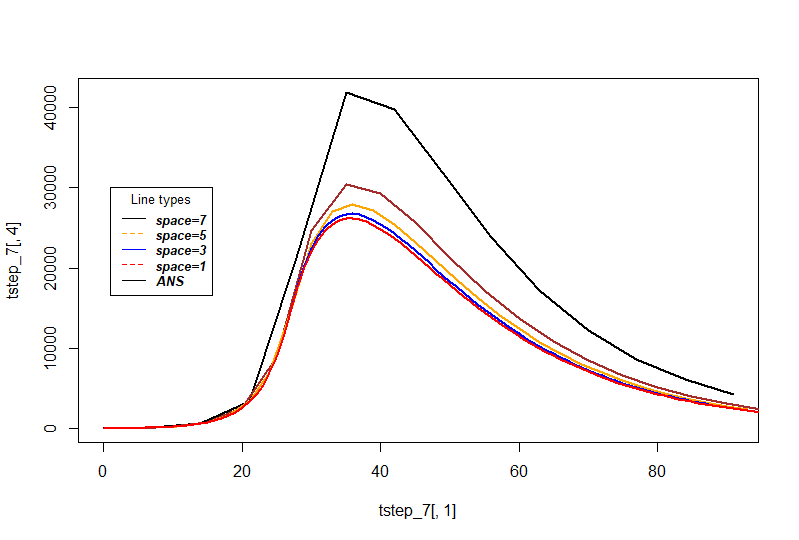
\includegraphics[width=0.7\linewidth]{./figures/R_ode45_spacing_experiment}
\caption{R `ode45' output point spacing experiment}
\label{fig:ode45_spacing_experiment}
\end{figure}

Figure $\ref{fig:ode45_spacing_experiment}$ shows an experiment where we solve the time discontinuity Covid-19 problem using the R `ode45' method, which is an implementation of DOPRI5 which has error control but does not use interpolation, to show that it is using more function evaluations than needed. We set both the absolute and relative tolerance to 0.1 and thus expect low accuracy but very good efficiency. However, the space between the points is still a limiting factor for the step-size and the solution is somewhat accurate although computed in a very inefficient manner. We recorded the number of function evaluations in Table $\ref{tab:ode45_spacing_experiment}$ and it can be seen that the solver is using a lot more function evaluations than are needed to satisfy such coarse tolerance. In Table $\ref{tab:ode45_spacing_experiment}$, `spacing' refers to the distance between the output points.

\begin{table}[h]
\caption {R DOPRI5 output point spacing experiment} \label{tab:ode45_spacing_experiment} 
\begin{center}
\begin{tabular}{ c c }
spacing & nfev \\ 
1 & 572 \\
3 & 188 \\
5 & 116 \\
7 & 80 \\
\end{tabular}
\end{center}
\end{table}

From Figure $\ref{fig:ode45_spacing_experiment}$ and Table $\ref{tab:ode45_spacing_experiment}$, we note that we did not ask the solver for an accurate solution but it is giving us an excessively accurate solution. This excess accuracy comes at a price of around 500 more function evaluations. Accuracy should ideally be completely determined by the tolerance but using this method of skipping to the output points substantially interferes with this ideal. This results in the solver not being allowed to take as big a step as it should be based on the tolerance, and this leads to substantial inefficiency. 

We advise users to use an interpolation option whenever readily available so that the solvers can run as efficiently as possible. We also reiterate that the interpolant should have an interpolation error that is at least of order $p$ if the ODE solver gives a solution with an error that is of order $p$ so that the interpolation error does not interfere with the accuracy of the numerical solution.

\subsection{Discontinuities and their effects on solvers}
\label{subsection:effect_of_discontinuity}
The main purpose of this report is to discuss how to solve models with discontinuities and how these discontinuities affect the process of computing an accurate numerical solution to the model. In this section, we will show what happens when a solver encounters a discontinuity and how this discontinuity leads to inaccurate solutions.

We first note that since all the solvers use numerical methods based on Taylor series, one of the core assumptions is that the function $f(t, y(t))$ and a sufficient number of its higher derivatives are continuous. If the right-hand side function is discontinuous, this can have a major (negative) impact on the performance and accuracy of the solvers. 

We will see that discontinuities will have huge impacts on the accuracy and efficiency of the solvers, that some solvers, even with error control, will require an extremely sharp tolerance to step over the discontinuity in a way that allows them to obtain a reasonably accurate solution approximation, and that fixed-step solvers simply cannot solve these problems accurately. 

It is important to note that the step that first meets a discontinuity will almost always fail. This is because for the code to step over a discontinuity, the step size needs to be much smaller than the one that is being used before the discontinuity. The codes will thus have to retake the step with a smaller step size and as long as the error estimate of the step is not small enough, it will need to continue reducing the step. This leads to high numbers of function evaluations near the discontinuity which will lead to larger CPU times. 

\begin{figure}[h]
\centering
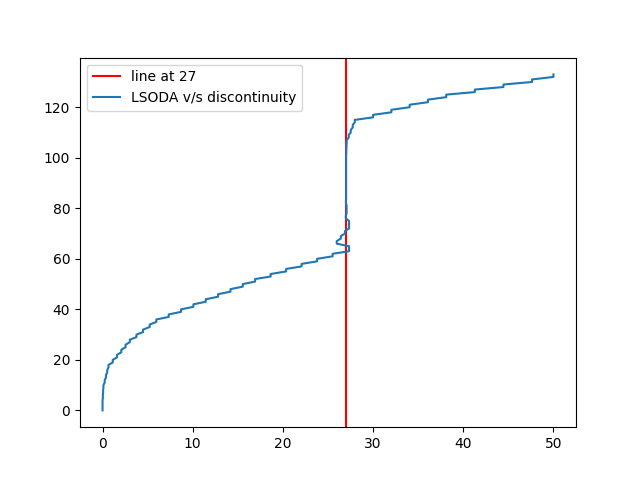
\includegraphics[width=0.7\linewidth]{./figures/lsoda_vs_discontinuity}
\caption{Function evaluations for the Python `LSODA' method for the time discontinuity method when there is a discontinuity at t=27}
\label{fig:lsoda_vs_discontinuity}
\end{figure}

\begin{figure}[h]
\centering
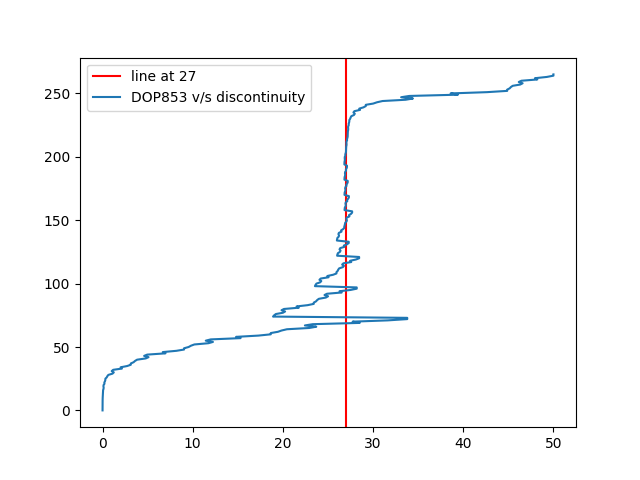
\includegraphics[width=0.7\linewidth]{./figures/dop853_vs_discontinuity}
\caption{Function evaluations for the Python `DOP853' method for the time discontinuity method when there is a discontinuity at t=27}
\label{fig:dop853_vs_discontinuity}
\end{figure}

In Figures $\ref{fig:lsoda_vs_discontinuity}$ and $\ref{fig:dop853_vs_discontinuity}$, we run `LSODA' and `DOP853' from Python on the time-dependent discontinuity problem where the discontinuity is introduced at t=27 and plot the time at which the $i^{th}$ function evaluation occurs. We thus show the spike in the number of function evaluations at the discontinuity as the solvers repeatedly retake the step with smaller and smaller step-sizes.

Following this discussion, we also recommend epidemiologists carry out a manual discontinuity detection experiment to see if their model has any discontinuity. This trivial experiment is done by collecting at what time the solver made the $i^{th}$ call to the solver. 

When a plot of the time against the cumulative count of the function calls gives an almost straight vertical line, it indicates that the function was called repeatedly at a specific time and thus that the solver repeatedly changed the step-size in this region to step over a discontinuity. In the remainder of this report, we will outline the ways to accurately and efficiently solve problems with such discontinuities.
